\documentclass[aspectratio=169,14pt,usenames,dvipsnames]{beamer}

\usepackage[utf8]{inputenc}
\usepackage{fontspec}
\usepackage{enumitem}
\usepackage{calc}

\usepackage{datetime}
\newcommand\builddate{%
   \ifcase \month%
        \or Janeiro%
        \or Fevereiro%
        \or Março%
        \or Abril%
        \or Maio%
        \or Junho%
        \or Julho%
        \or Agosto%
        \or Setembro%
        \or Outubro%
        \or Novembro%
        \or Dezembro%
    \fi\space\number\year%
}

\newcommand{\loadtheme}[1]{%
    \input{themes/#1}%
}
\newcommand{\presentationlanguage}[1]{%
    \usepackage[#1]{babel}%
}

\newcommand{\usecodingsamples}[1]{%
    \usepackage{listings}%
    \input{listings/#1}%
}

% Configura a apresentação para ser executada em tela cheia.
\newcommand{\setfullscreen}{\hypersetup{pdfpagemode=FullScreen}}

% Hide beamer navigation simbols
\beamertemplatenavigationsymbolsempty

%
% Standard frames
%

% coverframe
\newcommand{\coverframe}{%
    \begin{frame} %
        \titlepage %
    \end{frame} %
}

% finalframe{email}
\newcommand{\finalframe}[2][Thank you!]{%
    \begin{frame}%
        \begin{flushright}%
            \huge \textbf{#1}%
            \vfill%
            \large \textbf{#2}%
        \end{flushright}%
    \end{frame}%
}

% bigtitle{title}
\newcommand{\bigtitle}[1]{%
    \begin{frame}%
        \begin{center}%
            \Huge {#1}%
        \end{center}%
    \end{frame}%
}

% citation{cite}{author}
\renewcommand{\citation}[2]{%
    \begin{frame}%
        \begin{center}%
            \vspace{1cm}
            \large \textit{"#1"}\\%
            \vspace{1cm}
            \footnotesize {#2}%
        \end{center}%
    \end{frame}%
}

% bigimage{file}
\newcommand{\bigimage}[2][1.0]{%
    {%
        \usebackgroundtemplate{}%
        \begin{frame}%
            {%
            \makebox[\textwidth][c]{%
              \includegraphics[height=#1\paperheight, width=#1\paperwidth,%
                               keepaspectratio]{#2}%
              }%
            }%
        \end{frame}%
    }%
}


\loadtheme{photoroll}

\subtitle{Conceitos Básicos de Fotografia Digital}
\title{Formação da Imagem, Câmeras, Lentes e Controles Básicos}
\author{}
\institute{Rafael\textbf{Jeffman}\\\tiny{F O T O G R A F I A}}
\date{Abril de 2018}

\begin{document}

\coverframe

\begin{frame}
    \frametitle{A Formação da Imagem}
\begin{center}
    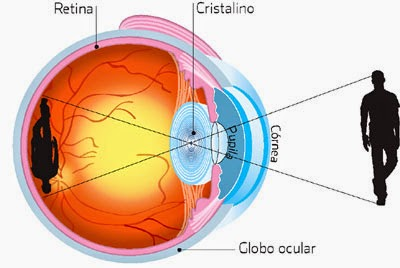
\includegraphics[height=6cm]{images/olho.jpg}
\end{center}
\end{frame}

\begin{frame}
    \frametitle{A Câmera Obscura}
\begin{center}
    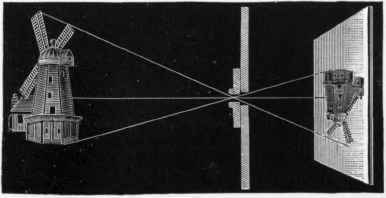
\includegraphics[height=7cm]{images/pinhole.jpg}
\end{center}
\end{frame}

\begin{frame}
    \frametitle{Joseph Nicéphore Niépce}
\begin{center}
    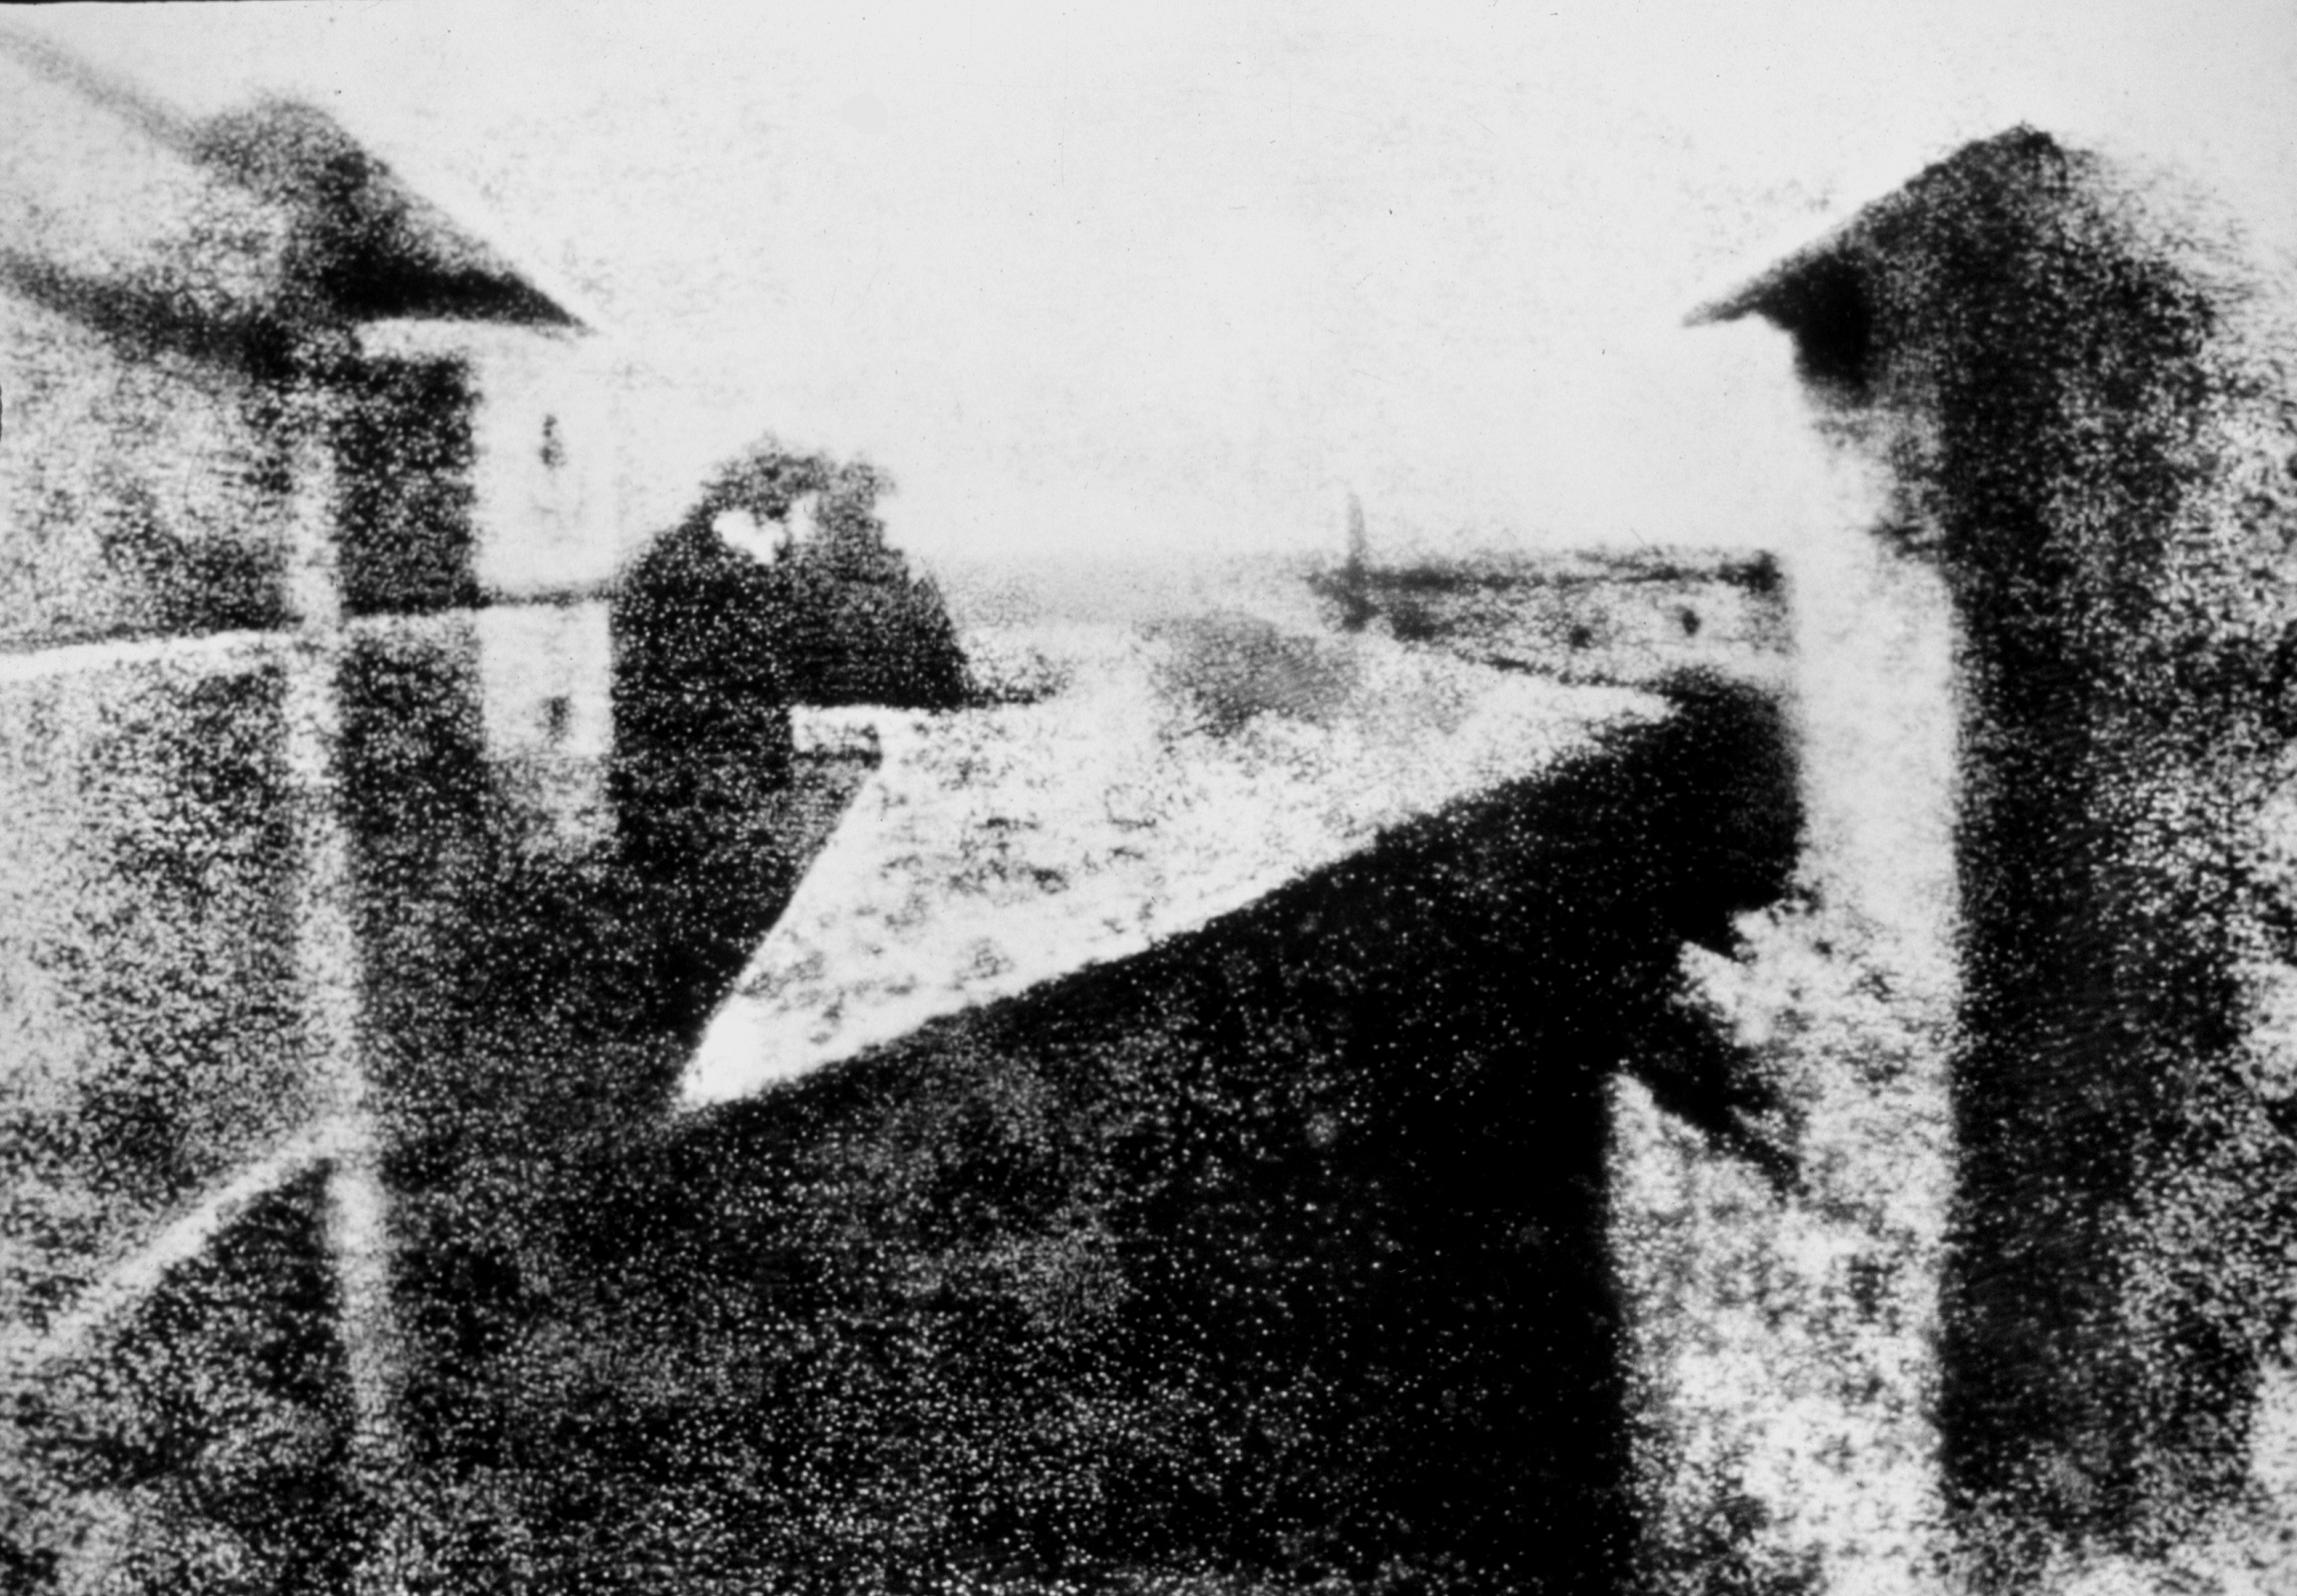
\includegraphics[height=7cm]{images/niepce.jpg}
\end{center}
\end{frame}

\begin{frame}
    \frametitle{Louis-Jaques-Mandé Daguerre}
\begin{center}
    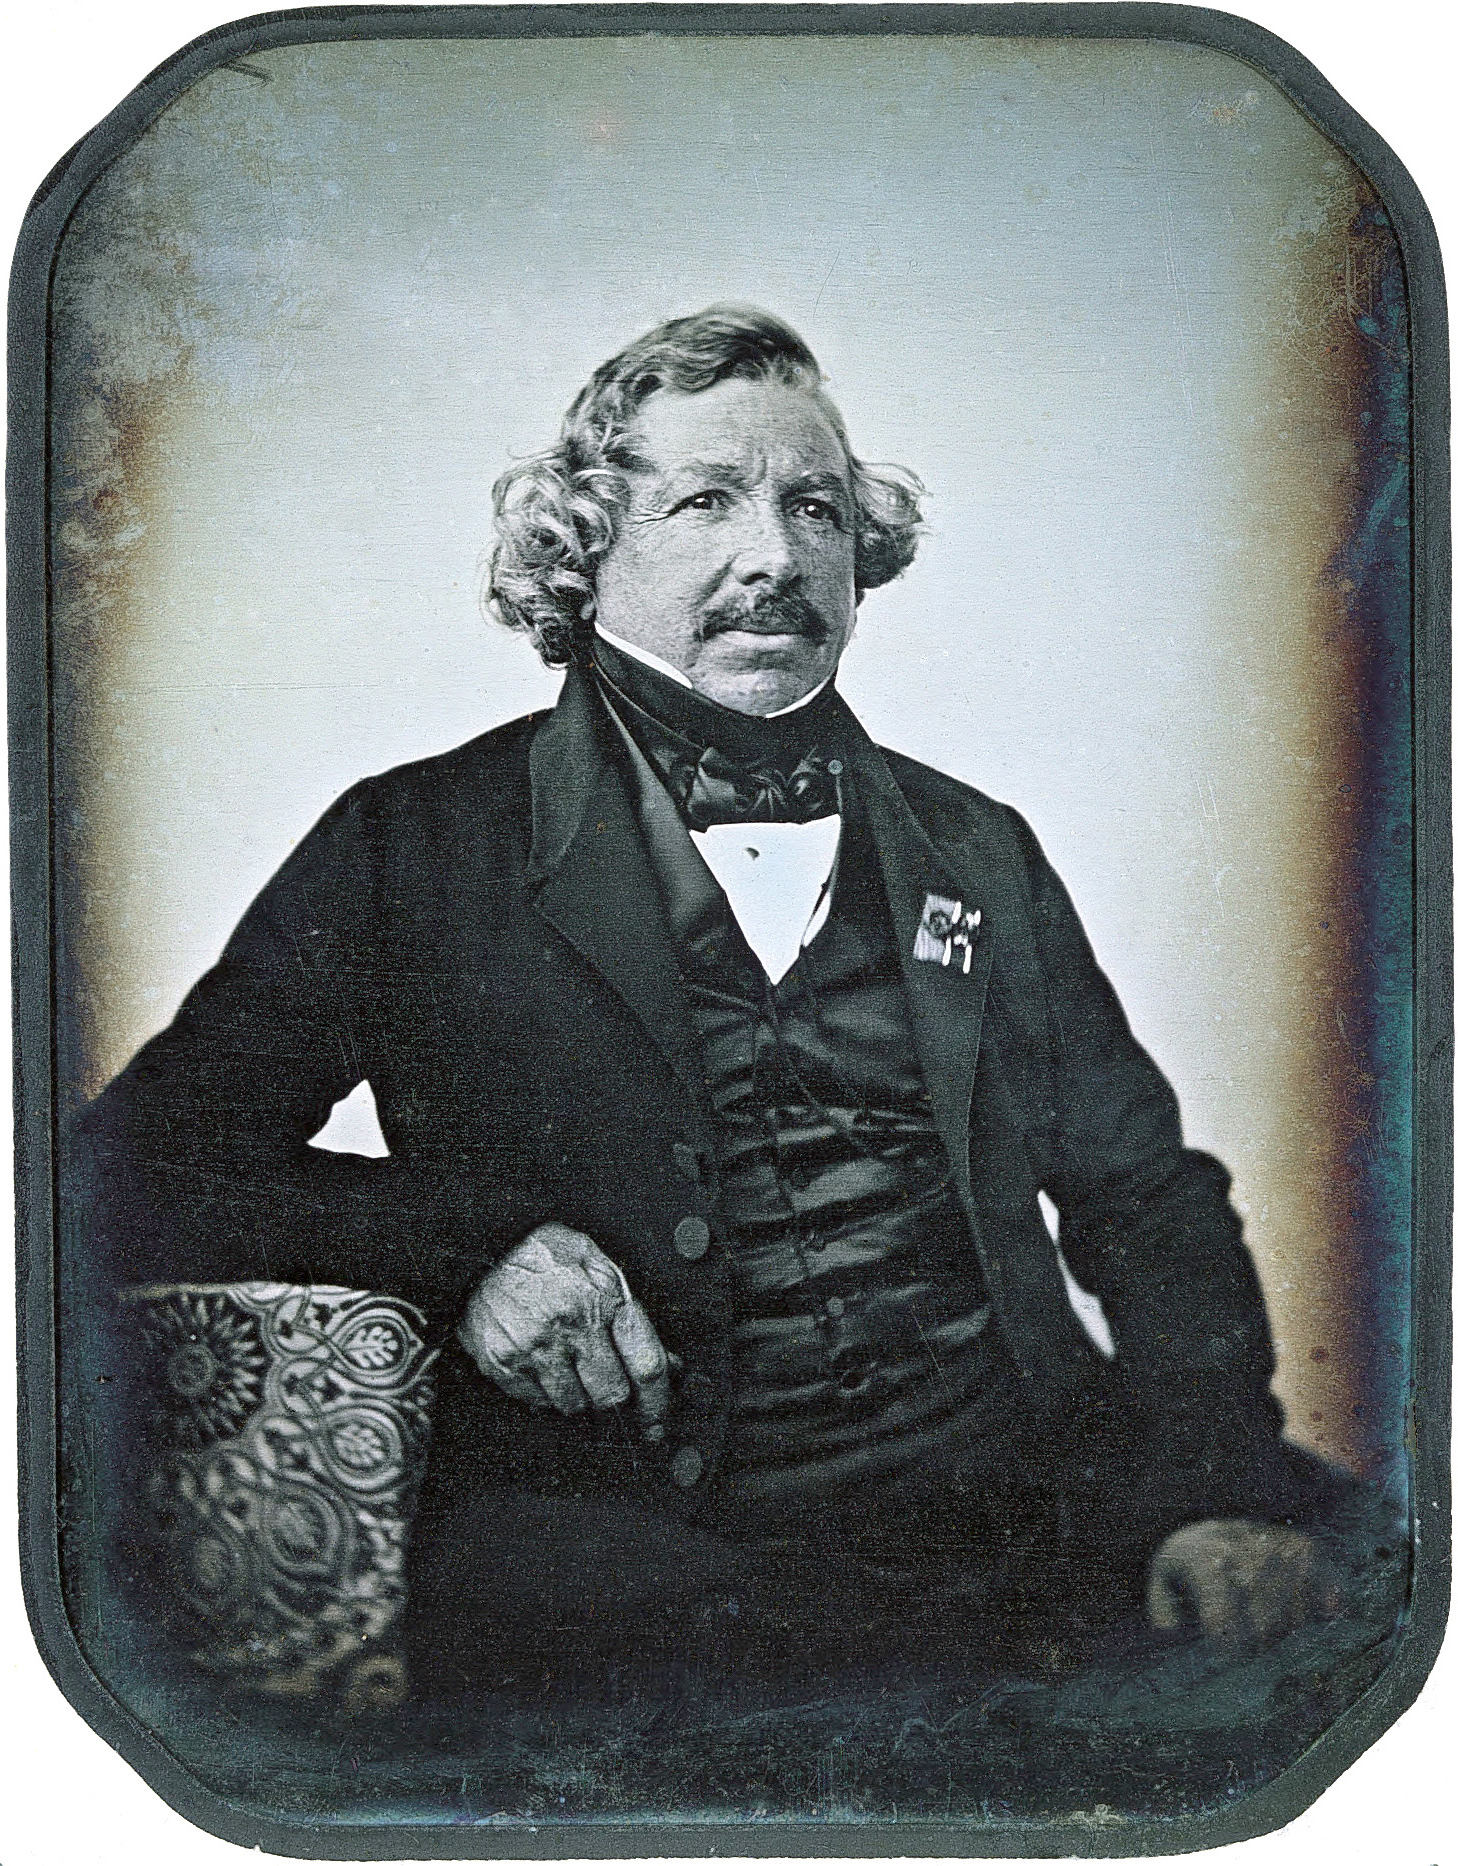
\includegraphics[height=7cm]{images/daguerre.jpg}
\end{center}
\end{frame}

\begin{frame}
    \frametitle{Hércule de Florence}
\begin{center}
    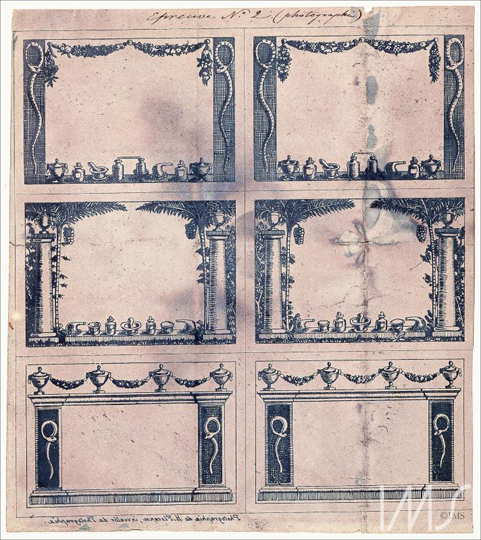
\includegraphics[height=7cm]{images/florence.jpg}
\end{center}
\end{frame}

\begin{frame}
    \frametitle{Câmera \textit{Pinhole}}
\begin{center}
    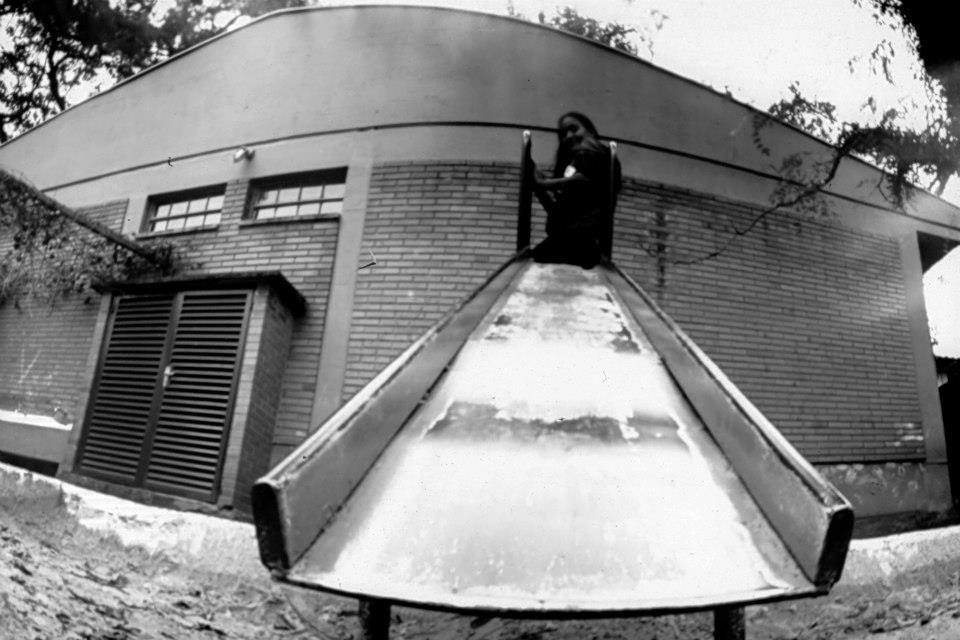
\includegraphics[height=7cm]{images/latamagica.jpg}
\end{center}
\end{frame}

\begin{frame}
    \frametitle{Formação da Imagem}
    \begin{itemize}
        \item Objeto Fotografado.
        \item Orifício para orientar a luz.
        \item Suporte sensível à luz.
    \end{itemize}
\end{frame}

\begin{frame}
    \frametitle{A Câmera Fotográfica}
\begin{center}
    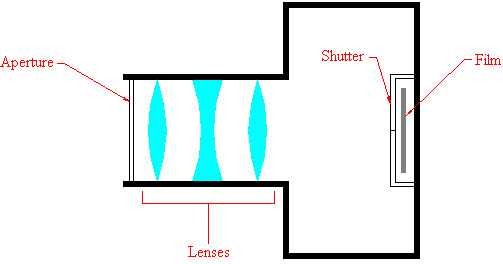
\includegraphics[height=7cm]{images/basic_camera.jpg}
\end{center}
\end{frame}

\begin{frame}
    \frametitle{Tipos de Câmeras}
    \begin{itemize}
        \item Celular
        \item Compactas / \textit{Point \& Shoot}
        \item Superzoom
        \item DSLR Reflex
        \item Médio Formato
        \item Técnicas
    \end{itemize}
\end{frame}

\imagehorizontal[\textit{Twin Lens Reflex}]{images/tlr.jpg}
\imagevertical[\textit{Alpa Technical Camera}]{images/alpa.jpg}
\bigimage{images/phaseone.jpg}
\bighorizontal{images/canon-nikon.jpg}

\bigtitle{Sensores Fotográficos}
\bigimage{images/sensorsizes.png}

\imagevertical[Matriz Bayer]{images/bayer.png}

\begin{frame}
        \frametitle{Sensores Digitais}

        \begin{itemize}
            \item Capturam uma cor por pixel.
            \item Os principais tipos são Matriz de Bayer, X-Trans e Foveon.
            \item Baseados em conversores analógicos digitais.
            \item Possuem uma sensibilidade base.
        \end{itemize}
\end{frame}

\begin{frame}
    \frametitle{Efeitos do sensor na fotografia}

    \begin{itemize}
        \item Sensibilidade à Luz.
        \item Ângulo de visão da objetiva.
        \item Tamanho dos fotosensores.
        \item Quantidade de pontos e resolução da imagem.
        \item Capacidade de reprodução de cores.
    \end{itemize}
\end{frame}

\begin{frame}
    \frametitle{Objetivas}
    \begin{itemize}
        \item Definem uma distância focal.
        \item Em conjunto com o sensor, definem um ângulo de visão.
        \item Permitem que uma grade quantidade de luz seja direcionada para o sensor.
        \item Possuem um limite máximo de entrada de luz, medido em relação à distância focal.
    \end{itemize}
\end{frame}

\imagevertical[\Large{Ângulo de Visão vs. Distância Focal}]{images/focal.jpg}
\imagevertical[\Large{Ângulo de Visão vs. Distância Focal}]{images/red-barn-sequence.jpg}

\begin{frame}
    \frametitle{Objetivas Normais}
    \begin{itemize}
        \item Ângulo de visão semelhante ao olho humano.
        \item O ângulo de visão varia entre 55$^o$ e 45$^o$
        \item As lentes fixas nessa faixa são, normalmente, bastante claras.
        \item Encontram-se nessa faixa as Objetivas:

        {\small \begin{itemize}
            \item Médio Formato: 70mm a 100mm
            \item 35 mm: 40mm a 55mm
            \item APS: 25mm a 35mm
        \end{itemize}}
    \end{itemize}
\end{frame}

\begin{frame}
    \frametitle{Objetivas Grande-angulares}
    \begin{itemize}
        \item Aumenta a extensão da cena capturada.
        \item Aumenta a percepção de perspectiva.
        \item O ângulo de visão varia entre $85^o$ e $55^o$
        \item Encontram-se nessa faixa as Objetivas:

        {\small \begin{itemize}
            \item Médio Formato: 45mm a 70mm
            \item 35 mm: 24mm a 35mm
            \item APS: 15mm a 25mm
        \end{itemize}}
    \end{itemize}
\end{frame}

\begin{frame}
    \frametitle{Objetivas Ultragrande-angulares}
    \begin{itemize}
        \item Permite uma forte manipulação de perspectiva.
        \item Tende a distorcer elementos próximos, nos cantos da imagem devido à perspectiva.
        \item O ângulo de visão varia entre $114^o$ e $90^o$
        \item Encontram-se nessa faixa as Objetivas:

        {\small \begin{itemize}
            \item Médio Formato: 28mm a 35mm
            \item 35 mm: 11mm a 21mm
            \item APS: 10mm a 14mm
        \end{itemize}}
    \end{itemize}
\end{frame}

\begin{frame}
    \frametitle{Objetivas Telefoto}
    \begin{itemize}
        \item Aumenta o tamanho relativo dos objetos, ao diminuir a extensão da cena capturada.
        \item Tende a comprimir os planos da cena.
        \item O ângulo de visão varia entre $12^o$ e $34^o$
        \item Encontram-se nessa faixa as Objetivas:

        {\small \begin{itemize}
            \item Médio Formato: 115mm a 400mm
            \item 35 mm: 70mm a 210mm
            \item APS: 45mm a 150mm
        \end{itemize}}
        \item Muitas vezes, se consideram as lentes até 85mm (35mm) como \textit{meia-tele}.
    \end{itemize}
\end{frame}

\begin{frame}
    \frametitle{Objetivas Super-telefoto}
    \begin{itemize}
        \item Capturam uma pequena fração do que um ser humano vê.
        \item Muito utilizadas para fotografar objetos muito distantes.
        \item O ângulo de visão varia entre $2^o$ e $8^o$
        \item Encontram-se nessa faixa as Objetivas:

        {\small \begin{itemize}
            \item Médio Formato: 500mm a 700mm (6$^o$)
            \item 35 mm: 300mm a 1200mm
            \item APS: a partir de 200mm
        \end{itemize}}
        \item Em uma APS, o ângulo de visão pode se aproximar de 1$^o$.
    \end{itemize}
\end{frame}

\imagevertical[Normal]{images/normal.jpg}
\imagevertical[Ultragrande-angular]{images/ultrawide.jpg}
\imagevertical[Meia-tele]{images/meia-tele.jpg}
\imagevertical[Super-telephoto]{images/supertele.jpg}

\begin{frame}
    \frametitle{Objetivas Especiais}
    \begin{description}
        \item[\textbf{Fisheye}] \hfill \\ Ângulo de visão extremo (180$^o$), sem manter as linhas retas.
        \item[\textbf{Macro}] \hfill \\ Focalização extremamente próxima e magnificação extrema.
        \item[\textbf{Correção de Perspectiva}] \hfill \\ Corrige convergência de perspectiva.
    \end{description}
\end{frame}

\imagevertical[Fisheye]{images/fisheye.jpg}
\imagevertical[Objetiva Macro]{images/macro-lens.jpg}
\imagevertical[Tubo Macro]{images/macro-tube.jpg}

\begin{frame}
    \frametitle{Focalização}
    \begin{itemize}
        \item Uma objetiva só pode focalizar, com precisão, em uma única distância.
        \item O foco pode ser utilizado como elemento de composição na fotografia.
        \item O foco pode ser realizado de forma manual ou automática.
        \item O foco automático pode ser continuo ou não, preditivo ou não.
        \item Ao escolher um ponto de foco automático, apenas aquele ponto será utilizado.
    \end{itemize}
\end{frame}

\begin{frame}
    \frametitle{Exposição ou Fotometria}
    \begin{itemize}
        \item Medição da quantidade de luz que irá atingir o sensor.
        \item Quanto mais luz atingir o sensor, mais clara será a foto.
        \item Uma foto muito clara pode perder detalhes pelo \textbf{estouro de altas luzes}.
        \item Quanto menos luz atingir o sensor, mais escura será a foto.
        \item Uma foto muito escura pode perder detalhes pelo \textbf{bloqueio de sombras}.
    \end{itemize}
\end{frame}

\begin{frame}
    \frametitle{Exposição "Correta"}

    \begin{itemize}
        \item Uma exposição "correta", mostra os brancos como brancos, e os pretos como pretos.
        \item Para obter uma exposição correta, basta saber quanta luz está incidindo na cena.
        \item O problema é que a câmera mede a cena a partir da luz refletida.
        \item Tentando resolver o problema, a câmera mede a cena como se fosse um \textit{cartão cinza 18\%}.
    \end{itemize}
\end{frame}

\imagevertical[Cartão Cinza, 18\%]{images/graycard}

\begin{frame}
    \frametitle{Controle de Exposição}
    Para controlar a exposição podemos alterar:
    \begin{itemize}
        \item A sensibilidade do suporte fotográfico.
        \item A quantidade de luz que atinge o suporte.
        \item O tempo que o suporte fica exposto à luz.
    \end{itemize}
\end{frame}

\bigimage{images/bucket-analogy.jpg}

\begin{frame}
    \frametitle{Controle de Exposição}
    \begin{itemize}
        \item Diversas configurações de Velocidade, Abertura e Sensibilidade geram a mesma exposição.
        \item Alterar a velocidade, abertura ou a sensibilidade causa diferentes efeitos à imagem.
    \end{itemize}
\end{frame}

\begin{frame}
    \frametitle{Controle de Exposição}
    \begin{itemize}
        \item Alterando a velocidade, altera-se também a nitidez e a sensação de movimento.
        \item Alterando a abertura, altera-se a profundidade de campo, diminuindo a distância hiperfocal.
        \item Alterando a sensibilidade, altera-se a quantidade de ruído e a capacidade de reprodução de cores.
    \end{itemize}
\end{frame}

\bigimage{images/exposure-triangle.jpg}

\imagevertical[ISO 100, 1/125, f:16]{images/graycard}
\imagevertical[ISO 400, 1/1000, f:11]{images/graycard}
\imagevertical[ISO 100, 1/500, f:8]{images/graycard}

\bigimage{images/black_white}

\begin{frame}
    \frametitle{Exposição Correta}
    Expor corretamente significa escolher o objeto mais importante da cena e
    ajustar a esposição de forma que este objeto seja mostrado como desejado.
\end{frame}

\begin{frame}
    \frametitle{O Obturador}
    \begin{itemize}
        \item Controla o \textbf{tempo} de exposição.
        \item Expõe o suporte sensível à luz.
        \item Pode não expor totalmente o suporte.
        \item Controla "quanto de movimento" é capturado.
    \end{itemize}
\end{frame}

\begin{frame}
    \frametitle{O Tempo de Exposição.}
    \begin{itemize}
        \item Medido em $1/t$ segundos.
        \item Se for muito rápido, congela o movimento.
        \item Se for muito lento, pode permitir fotos tremidas ou objetos borrados.
        \item Pode ser utilizado para gerar efeitos como \textit{panning} ou movimento em líquidos.
    \end{itemize}
\end{frame}

\begin{frame}
    \frametitle{A Escala de Tempo}
    \vfill
    \begin{center}
    \mbox{
    \huge $1$
    \hfill
    \huge $\frac{1}{2}$
    \hfill
    \huge $\frac{1}{4}$
    \hfill
    \huge $\frac{1}{8}$
    \hfill
    \huge $\frac{1}{15}$
    \hfill
    \huge $\frac{1}{30}$
    \hfill
    \huge $\frac{1}{60}$
    \hfill
    \huge $\frac{1}{125}$
    \hfill
    \huge $\frac{1}{250}$
    \hfill
    \huge $\frac{1}{500}$
    \hfill
    \huge $\frac{1}{1000}$
    }
    \end{center}
    \vfill
\end{frame}

\begin{frame}
    \frametitle{Tempos comuns de exposição.}
    \begin{itemize}
        \item Retratos parados: 1/60
        \item Pessoas caminhando: 1/125
        \item Atividades Esportivas: 1/400 - 1/2000
        \item \textit{Panning}: 1s - 1/30
        \item Fotografia de Estrelas: 30s a várias horas...
    \end{itemize}
\end{frame}

\bigimage{images/confete.jpg}
\bigimage{images/tenis.jpg}
\bigimage{images/helicopter.jpg}
\bigimage{images/vialactea.jpg}

\begin{frame}
    \frametitle{O Diafragma}
    \begin{itemize}
        \item Define a \textbf{abertura} da lente.
        \item Limita a quantidade de luz que passa pela lente.
        \item Controla a profundidade de campo.
        \item Afeta a ordenação dos raios de luz.
    \end{itemize}
\end{frame}

\begin{frame}
    \frametitle{O Diafragma}
    \begin{itemize}
        \item É composto por "lâminas".
        \item É medido em "$f$-stops".
        \item Cada vez que permite a passagem de metade da luz, o número
              cresce à proporção da $\sqrt{2}$.
        \item É definido em termos da distância focal: $f=\frac{DF}{A}$
    \end{itemize}
\end{frame}

\imagehorizontal[A Escala do Diafragma]{images/diafragma.jpg}
\imagehorizontal[Diafragma $f$:16]{images/f16.jpg}
\imagehorizontal[Diafragma $f$:5.6]{images/f5-6.jpg}
\imagehorizontal[Diafragma $f$:1.4]{images/f1-4.jpg}

\begin{frame}
    \frametitle{Uso criativo do diafragma.}
    \begin{itemize}
        \item A maioria das lentes possui sua melhor condição ótica com o diafragma fechado em um ou dois pontos.
        \item Ao fechar muito o diafragma, a nitidez da imagem é reduzida devido ao efeito de difração.
        \item Utilizando a lente totalmente aberta, permite selecionar o que estará em foto na imagem.
        \item É possível criar efeitos especiais, utilizando artefatos a frente da lente e desfocando
        luzes na imagem.
    \end{itemize}
\end{frame}

\imagehorizontal[Foto Seletivo]{images/foco_seletivo.jpg}
\imagehorizontal[\textit{Bokeh} com Formas]{images/bokeh_shapes.jpg}

\begin{frame}
    \frametitle{A Sensibilidade a Luz}
    \begin{itemize}
        \item Define quanto de luz é necessário para obter a imagem.
        \item Quanto maior a sensibilidade, maior a quantidade de ruído.
        \item Quanta maior a sensibilidade, menor a capacidade de reprodução de cores.
    \end{itemize}
\end{frame}

\begin{frame}
    \hspace{0.5cm}baixo\hspace{0.5cm}normal\hspace{2cm}alto\hspace{3cm}muito alto
    \frametitle{Escala ISO}
    \vfill
    \begin{center}
    \mbox{
    \large 25
    \hfill
    \large \texttt{50}
    \hfill
    \large \textbf{100}
    \hfill
    \large \textit{200}
    \hfill
    \large 400
    \hfill
    \large 800
    \hfill
    \large 1600
    \hfill
    \large 3200
    \hfill
    \large 6400
    \hfill
    \large 12800
    \hfill
    \large 25600
    \hfill
    }
    \end{center}
    \vfill
\end{frame}

\finalframe[Vamos gastar o obturador!]{rafasgj@gmail.com}

\end{document}
